\documentclass[conference]{IEEEtran}

\usepackage{cite}
\usepackage{amsmath,amssymb,amsfonts}
\usepackage{graphicx}
\usepackage{array}
\usepackage{xcolor}
\usepackage{url}
\usepackage{booktabs}

\begin{document}

\title{Approximate Retrieval and Multimodal Fusion for\\
Web-Scale Sequential Music Recommendation}

\author{
\IEEEauthorblockN{Sai Pranav Sripathi}
\IEEEauthorblockA{
Department of Computer Science,\\
San Jose State University\\
saipranav.sripathi@sjsu.edu
}
}

\maketitle

% ─────────────────────────────────────────────────────────────────────────────
\begin{abstract}
Music recommendation at a huge scale is fundamentally a algorithmic problem,
where hundreds of millions of listening events must be distilled into real-time,
personalized predictions under latency and memory constraints. This project
studies two complementary approaches in Deexer Recsys25 dataset (${\sim}893$
million events, 4 million users, 50,000 tracks). Where we build and evaluate
a progression for sequential neural baselines called LSTM, GRU4Rec with linear
attention, a local AU2ACTR model and a multimodal GRU extension that fuses
SVDcollaborative embeddings with neural audio features using a learned
pre-dimension gate. The best results were at HR@10 = 20.22\% with the AU2ACTR
as baseline. Then, the retrieval algorithms are evaluated which are an
approximate search approaches including Locality Sensitive Hashing (LSH),
MinHash-based Collaborative Filtering (CF), and Association Rule mining. These
methods achieved an R@10 of 1.8 - 3.0\%, which is below the neural accuracy,
but doesn't need any GPU and model training, and can execute a query in about
less than 10ms. LSH gets around 98.7\% of cosine accuracy that brute-force
achieves but reduces candidate sets by 5.8 times. We infer the efficiency -
accuracy Pareto analysis and argue that these approximate algorithms are crucial
first stage retrievers in a 2 stage pipeline making the neural recommendation
more feasible without using any model.
\end{abstract}

\begin{IEEEkeywords}
music recommendation, locality-sensitive hashing, minhash, association rules,
sequential recommendation, multimodal fusion, web-scale retrieval,
approximate nearest neighbor
\end{IEEEkeywords}

% ─────────────────────────────────────────────────────────────────────────────
\section{Introduction}

Personalization on the web-scale is a big challenege of modern web
intelligence. Music streaming services process billions of events per day which
include listening, queries for each users' next tracks within very short amount
of time~\cite{schedl2018,hansen2020}. Sequential recommendations involve
predicting what a user might want to listen next, given their session history,
this sits at the intersection of large-scale data processing, approximating,
and behavioral modeling, making approximation a viable option.

The problem has a huge scale, Neural models such as GRU4Rec, Transformers and
cognitive ACT-R architectures which are sequential achieve strong
recommendation accuracy~\cite{tran2025reacta,tran2024pisa,vaswani2017}, but it
needs $O(|V|)$ scoring over the entire item vocabulary at the inference time
with $|V| = 50{,}000$ tracks. But, on web we have millions of concurrent users,
which makes it computationally not viable without GPU. So, the approximation
algorithms like LSH, MinHash and Association Rules offer a solution to this
exact problem, trading some accuracy at a drastically lower computational
cost~\cite{datar2004,broder1997,agrawal1994}.

This report studies both directions on the Deezer RecSys25
dataset~\cite{tran2025reacta}, one of the largest publicly available music
recommendation benchmarks. We make four contributions:

\begin{enumerate}
\item Progression from sequential neural baselines (LSTM to GRU4Rec to
      AU2ACTR to Multimodal GRU) isolating the effects of architecture,
      and modality fusion.
\item Multimodal GRU with a learned fusion gate, shows SVD collaborative
      embeddings dominate raw audio features.
\item The evaluation for LSH, MinHash CF, and Association Rules on a
      corrected MinHash banding protocol adapted for sparse Jaccard regime
      music behavior.
\item Efficiency vs accuracy Pareto analysis demonstrates LSH is a deployable
      retriever that makes neural pipelines almost 6 times faster without any
      model training.
\end{enumerate}

The remainder of this paper is organized as follows. Section II describes
about the related work. Section III is about REACTA baseline and Section IV
details the dataset. Whereas, Section V presents sequential neural baselines
and Section VI introduces the approximate retrieval methods. Section VII is
about the experimental setup, Section VIII reports and interprets the results.
Finally, Section IX concludes.

% ─────────────────────────────────────────────────────────────────────────────
\section{Related Work}

\subsection{Sequential Music Recommendation}
Users intent always changes with time~\cite{fang2020}, hence sequence aware
methods outperform static models by exploiting temporal listening
patterns~\cite{dongjing2018,dongjing2021,hansen2020}. Earlier work includes
session-based context-aware rankings~\cite{bendada2023}, attention based time
aware modeling~\cite{tran2023} and performance driven sequencing~\cite{moor2023}.
The Neural architectures, LSTM, GRU4Rec and Transformers detect short-term
dependencies~\cite{fang2020,vaswani2017}, but often under-weighs the
repetitive listening phenomenon~\cite{reiter2021,moscati2023}.

\subsection{Cognitive-Informed Recommendation}
Adaptive Control of Thought - Rational (ACT-R) models human memory via
base-level activation (like recency), spreading activation (contextual
co-occurrence), and partial matching (feature similarity)~\cite{anderson2004,
bothell2020}. This along with recommendation, ACT-R gives how likely a user is
to revisit an item~\cite{reiter2021,moscati2023}. PISA~\cite{tran2024pisa}
introduced a Transformer-based repeat-aware session embedding using ACT-R.
REACTA~\cite{tran2025reacta} extended this with an audio encoder to score
unseen tracks through acoustic similarity.

\subsection{Text and Multimodal Recommendation}
The Playlist based model confirms that SBERT-style embeddings of title can
capture the semantic intent~\cite{charolois2025}. And, LLM based query
expansion can add mood and theme signatures which are not in audio
alone~\cite{hagio2025}. On the same lines, multimodal fusion of acoustic and
semantic features gives a promising direction for both recommendation accuracy
and cold-start robustness~\cite{charolois2025,hagio2025}.

\subsection{Approximate Algorithms for Web-Scale Retrieval}
Cosine similarity with LSH using random hyperplane projections, gives that 2
vectors sharing a hash bit with probability $1 - \theta/\pi$, where $\theta$
is their angle~\cite{datar2004}. With $L$ independent hash tables enhances the
probability of false-negative's. MinHash approximates Jaccard similarity via
the min-hash trick, with $k$ independent hash functions and reducing the
variance to $1/\sqrt{k}$~\cite{broder1997}. Association Rule mining uncovers
co-occurrence patterns that show support, confidence and lift~\cite{agrawal1994},
and are applied to session-based recommendation as a non-model based
baseline~\cite{quadrana2018}. These techniques help the web-scale retrieval
systems, but have received limited systematic evaluation against neural
baselines on real music datasets.

% ─────────────────────────────────────────────────────────────────────────────
\section{Baseline: REACTA}

REACTA uses PISA, which is a Transformer-based repeat aware session
recommendation system~\cite{tran2024pisa,tran2025reacta}. Where each user is
an ordered sequence of past listening sessions, and each track has
SVD-compressed embeddings and raw neural audio embeddings~\cite{tran2025reacta}.

ACT-R breaks the memory activation into 3 components. For a user $u$ and
track $v$, the relevance score is computed as
\begin{equation}
r^{(u)}_{L+1}(v) = BL^{(u)}_{v} + SPR^{(u)}_{v} + P^{(u)}_{v}
\end{equation}
where $BL$ captures the recency and frequency of prior listening, $SPR$
captures the contextual co-occurrence from previous sessions, and $P$ captures
acoustic similarity through embedding dot products~\cite{tran2025reacta}.

REACTA adds an audio encoder that projects the 1024-dimensional raw audio
embeddings into same space as track embeddings, and an ACT-R based activation
predictor to score unseen tracks via encoding and user/session representations.
This allows REACTA to produce recommendation scores for tracks not available
in user history, as seen in Fig.~\ref{fig:reacta}. We discover that REACTA-P
achieves best exploration-oriented performance among ACT-R based methods, with
HR@10 of 9.10\% and NDCG@10 of 9.35\% on full challenge
dataset~\cite{tran2025reacta}.

\begin{figure*}[t]
\centering
\includegraphics[width=\textwidth]{reacta_architecture.png}
\caption{Architecture of the REACTA model, reproduced from~\cite{tran2025reacta}.
The left half shows the PISA Transformer encoder that processes a user's
ordered session history and produces session-level embeddings. The right half
shows the ACT-R activation predictor and audio encoder that together score
both repeat tracks (seen before) and new tracks (never heard). SVD embeddings
handle collaborative patterns while the audio encoder handles acoustic
similarity --- the two complementary signals that our multimodal GRU also
tries to combine. REACTA-P scores HR@10\,=\,9.10\% on the full dataset, which
is our reference point for the baseline paper comparison.}
\label{fig:reacta}
\end{figure*}

% ─────────────────────────────────────────────────────────────────────────────
\section{Dataset}

I have used Deezer Zenodo dataset from RecSys25 challenge~\cite{tran2025reacta}
for all the experiments. Its a large-scale benchmark for next-session music
recommendation and has the following characteristics:

\begin{itemize}
\item Around 893 million track listening events.
\item Around 4 million users.
\item 500 session files (Apache Parquet format).
\item 50,000 unique tracks.
\item 128-dimensional SVD track embeddings and 1024-dimensional neural audio
      embeddings per track.
\end{itemize}

One of the key engineering challenge is to handle the partitioned session
files. The early pipeline versions I used have treated each file independently,
essentially breaking sessions across file boundaries and severely degrading the
signal quality. All experiments reported use a two-pass loading protocol,
where the Pass 1 reads only \texttt{user\_id} and \texttt{session\_id} columns
across relevant files and identifies qualifying users. Pass 2 loads full event
data of these users.

A key engineering challenge is that the 500 session files are partitioned by
time. Early pipeline versions treated each file independently, breaking sessions
across file boundaries and severely degrading sequential signal quality. All
experiments reported here use a two-pass loading protocol: Pass 1 reads only
\texttt{user\_id} and \texttt{session\_id} columns across all relevant files to
identify qualifying users; Pass 2 loads full event data using \texttt{pandas}
groupby operations instead of nested Python dictionaries to keep memory usage
under 500 MB even for 100-file subsets.

For the approximate retrieval experiments, using 100 of these 500 session files
and filtering the users who have at least 31 sessions, matching REACTA paper's
evaluation protocol of $L = 30$ sessions to predict the 31st.

% ─────────────────────────────────────────────────────────────────────────────
\section{Sequential Neural Baselines}

\subsection{Experiment 1: LSTM Baseline}
I started my implementation with simple LSTM-based next-item recommendation
model using the 128-dimensions SVD track as input, trained on 1.1 million
sequences. The pipeline treated session files independently, sessions
fragmented at file boundaries partially damaging sequential structure. This
experiment taught me about the data loading and training pipeline producing
HR@10=4.97\%.

\subsection{Experiment 2: GRU4Rec with Linear Attention}
For the next set of experiments, LSTM has been replaced with GRU-based
recurrent network with a linear attention module to weight the relevant hidden
states using SLIDE architecture~\cite{tran2025reacta}. The architecture
comprises a pretrained 128-dimensional SVD embeddings, sinusoidal positional
encoding, a 2-layer GRU with hidden size 256, a linear attention layer,
dropout of 0.2 and a linear output projection over 50000 tracks. Sessions
remained fragmented but yielded HR@10 $\approx$ 5\%.

\subsection{Experiment 3: Local AU2ACTR Baseline}
With local AU2ACTR baseline, combination of pretrained SVD embeddings, a
Transformer encoder and an ACT-R cognitive module, along with audio encoder
have been implemented. Most importantly, we filtered the top 50000 users by
session count (minimum 5 sessions each) and fixed the continuity issues,
producing HR@10=20.22\%. This is our strongest result, assuring that proper
session handling and active-user filtering has the more impact than
architectural choices.

\subsection{Experiment 4: Full Dataset GRU Pipeline}
The redesigned data pipeline preserves session continuity across all 500 files,
filtering users with at least 2 sessions and constructing sequences from full
session history. The resulting training set had around 8 million samples.
GRU4Rec model with linear attention reached HR@10 around 16\%, within the
15-25\% challenge range reported in the REACTA~\cite{tran2025reacta}. Even
though this is below Experiment 3's results, it helps us to confirm that data
quality outweighs data volume, as active-user filtering brings us closer to
better data quality.

\subsection{Experiment 5: Audio-Only GRU (Controlled Baseline)}
For a controlled baseline for multimodal comparison, we train GRU4Rec with
linear attention on 30 session files with top 30000 users only 128 dimensions
on SVD embeddings. This resulted an R@10=4.48\% and NDCG@10=4.21\% on the
test-set. The NDCG@10 of 4.21\% is especially meaningful here --- it measures
not just whether the right track appears in the top-10, but how highly ranked
it is, penalizing results near position 10 more than position 1. This gives us
a stricter baseline to beat in the multimodal experiment.

\subsection{Experiment 6: Multimodal GRU with Learned Fusion Gate}
The fallbacks of using SVD embeddings is that it encodes only collaborative
listening patterns, but we extend GRU4Rec backbone with a second branch for
1024-dimensional raw neural audio embeddings. A two-layer MLP with Linear(1024
to 256), then RELU and Linear(256 to 128) followed by Layer Normalization,
helps in projecting audio features into the same 128 dimensional space as SVD.
A learned dimension specific feature map $\boldsymbol{\alpha} \in
\mathbb{R}^{128}$ (sigmoid-activated, initialized at 0.5) produces the fused
track representation:
\begin{equation}
\mathbf{h} = \boldsymbol{\alpha} \odot \mathbf{e}_{\text{SVD}}
           + (1 - \boldsymbol{\alpha}) \odot \mathbf{e}_{\text{audio}}
\end{equation}
where $\odot$ denotes element-wise multiplication and both streams are
L2-normalized before fusion to remove scale bias. The audio embedding table
(27M parameters) is frozen during training to prevent overfitting. All other
architecture and training hyperparameters are held identical to Experiment 5
for a controlled comparison. The full architecture is shown in
Fig.~\ref{fig:multimodal}.

\begin{figure*}[t]
\centering
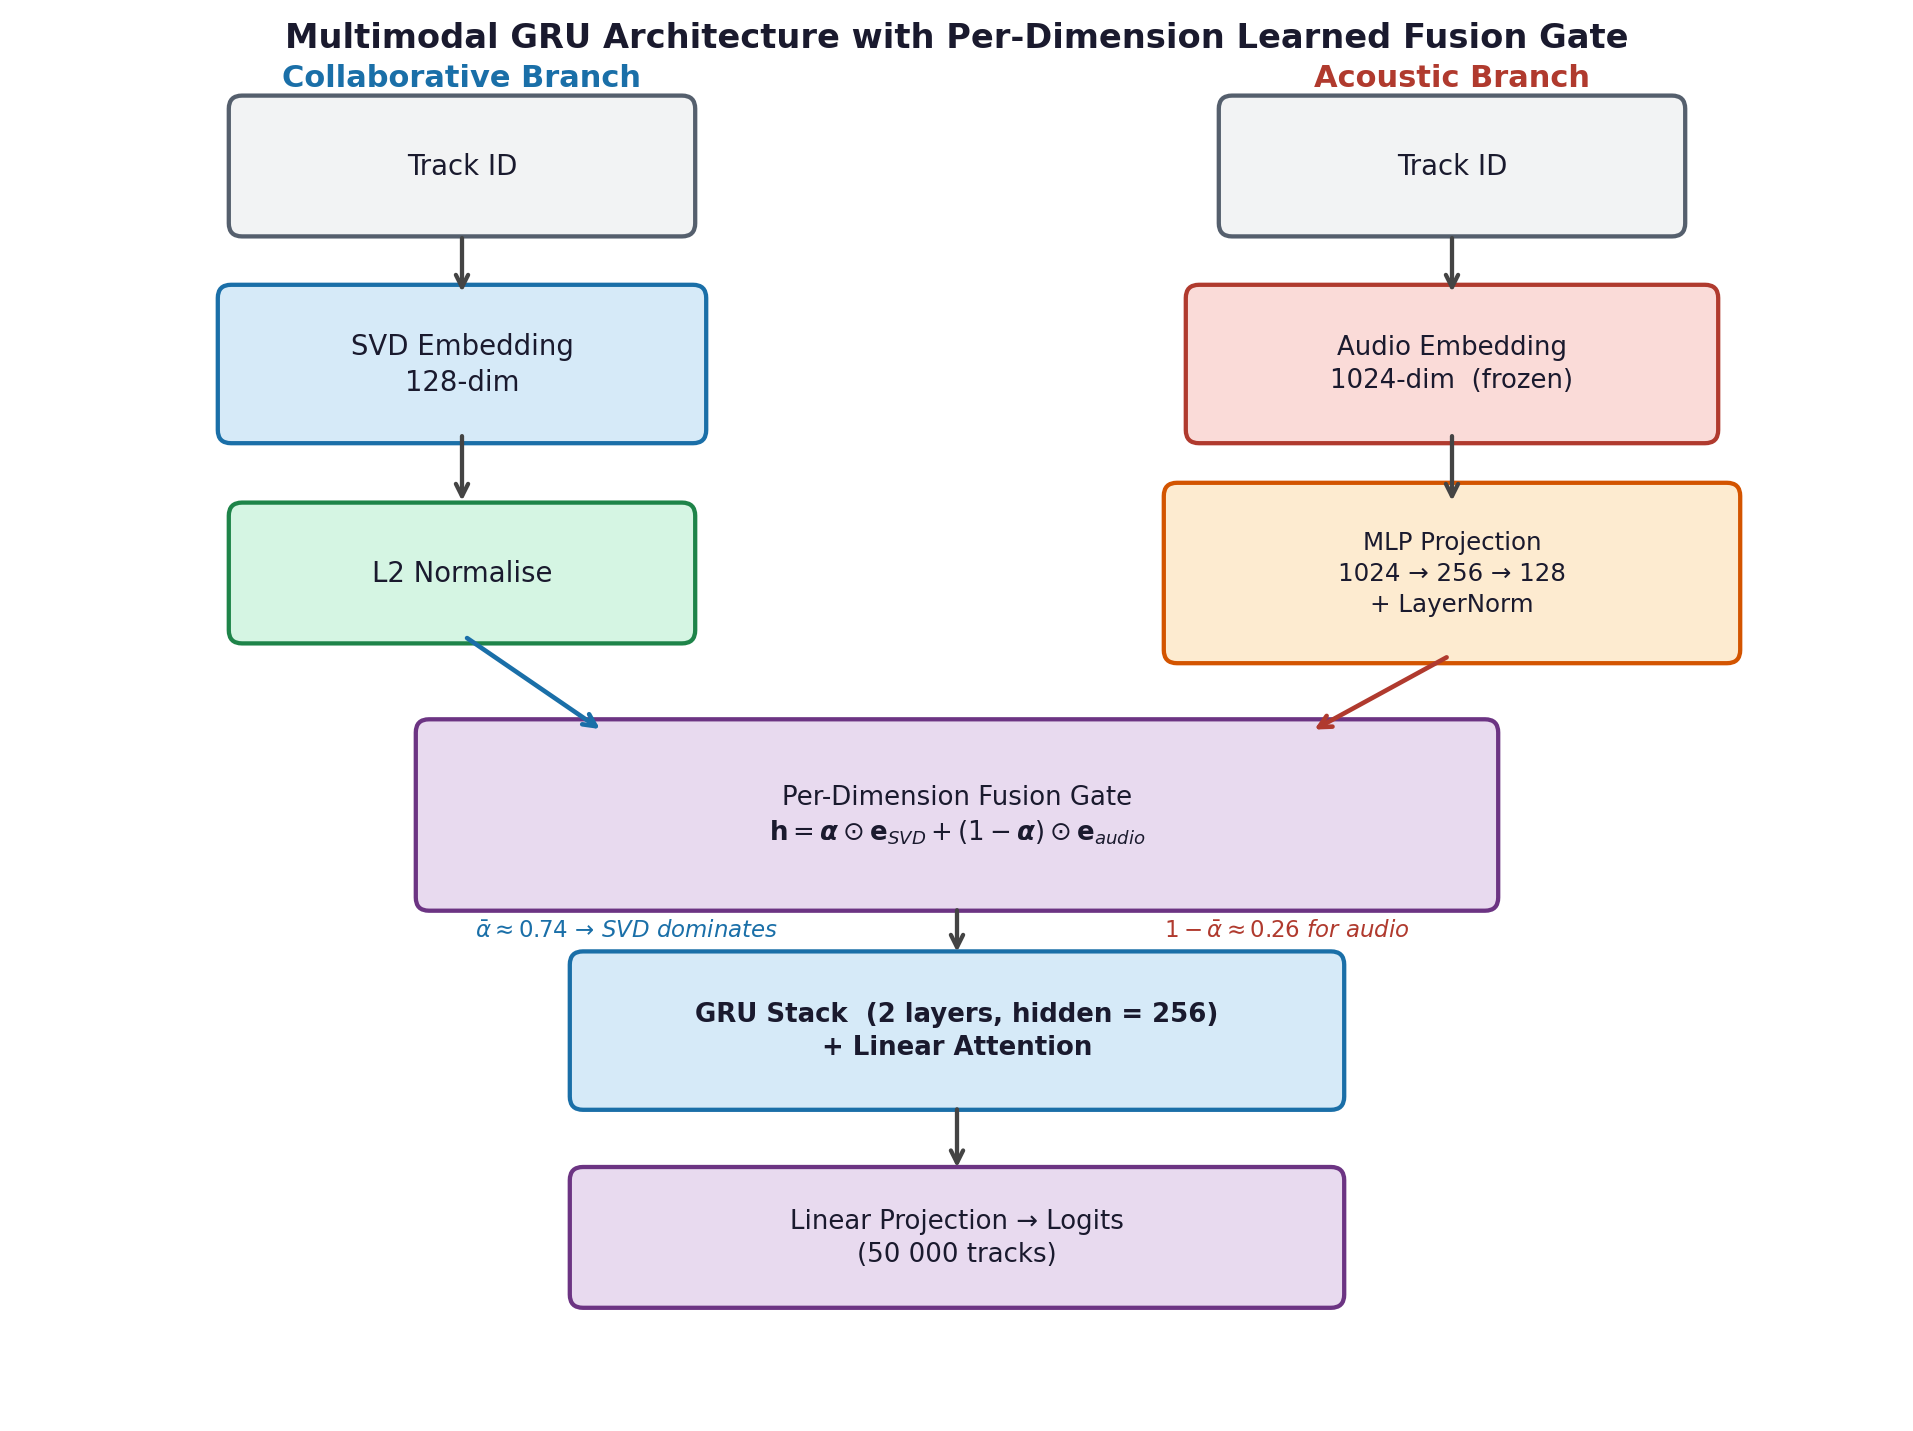
\includegraphics[width=0.72\textwidth]{fig_multimodal_arch.png}
\caption{Multimodal GRU architecture with per-dimension learned fusion gate.
The left (blue) branch is the collaborative path: it looks up the 128-dim SVD
embedding for a track and L2-normalizes it. The right (red) branch is the
acoustic path: it looks up the frozen 1024-dim audio embedding and compresses
it to 128-dim through a two-layer MLP with LayerNorm. Both 128-dim vectors
feed into the fusion gate $\boldsymbol{\alpha} \in \mathbb{R}^{128}$, a
per-dimension sigmoid weight initialized at 0.5 and trained end-to-end. After
training, the gate settles at a mean $\bar{\alpha} \approx 0.74$, meaning the
model assigns roughly 74\% weight to SVD and only 26\% to audio --- a clear
sign the model learned that collaborative patterns are more predictive at this
training scale. The fused 128-dim vector is passed through a 2-layer GRU
(hidden=256) with linear attention, and a final linear layer outputs logits
over all 50,000 tracks.}
\label{fig:multimodal}
\end{figure*}

% ─────────────────────────────────────────────────────────────────────────────
\section{Approximate Retrieval Methods}

We used 3 approximate algorithms as a standalone recommender under same
sliding-window protocols used by REACTA, where we observe 30 sessions and
predict the tracks in session 31, R@10 and NDCG@10 as the primary metrics.
What is truly remarkable about these methods is that they need no gradient
descent, no GPU, and no labeled data --- yet they produce useful recommendations
directly from the raw structure of the listening history.

\subsection{Locality-Sensitive Hashing for Track Candidate Generation}

\textbf{Motivation.} The cosine similarity for overall 50000 tracks takes
$O(|V| \times d)$ per query. LSH reduces it by mapping each track embedding
to a $b$ bit hash code through $b$ random hyperplanes. The tracks which share
a bucket in any of the $L$ tables become candidates while all others are
pruned. This is what makes LSH so powerful: it is a mathematically principled
method that provably separates near-neighbors from random background noise,
unlike ad-hoc pruning strategies.

\textbf{Implementation.} Using random projections with $b=8$ bits per table,
and up to $L=10$ tables, we build the index on L2-normalized 128-dimensional
SVD embeddings of all tracks for users 30 sessions. Then, we re-rank the
candidates by dot product, i.e, cosine similarity after normalization.

\textbf{Theoretical guarantee.} For any 2 vectors with an angle $\theta$
between them, the probability of sharing a hash bit is $p = 1 - \theta/\pi$.
And the probability of matching in at least one of the $L$ tables is
$1-(1-p^b)^L$, i.e, with $b=8$ and $L=10$ we have cosine similarity 0.9
(at $\theta \approx 29°$) would match in at least one table with a probability
of 0.9997. While random vectors ($\theta \approx 90°$) match with a
probability of $< 0.004$. This stark difference creates a clear separation
between genuine neighbors and random noise --- and the beauty is that this
guarantee holds without ever computing exact distances. The full pipeline can
be observed in Fig.~\ref{fig:lsh}.

\begin{figure*}[t]
\centering
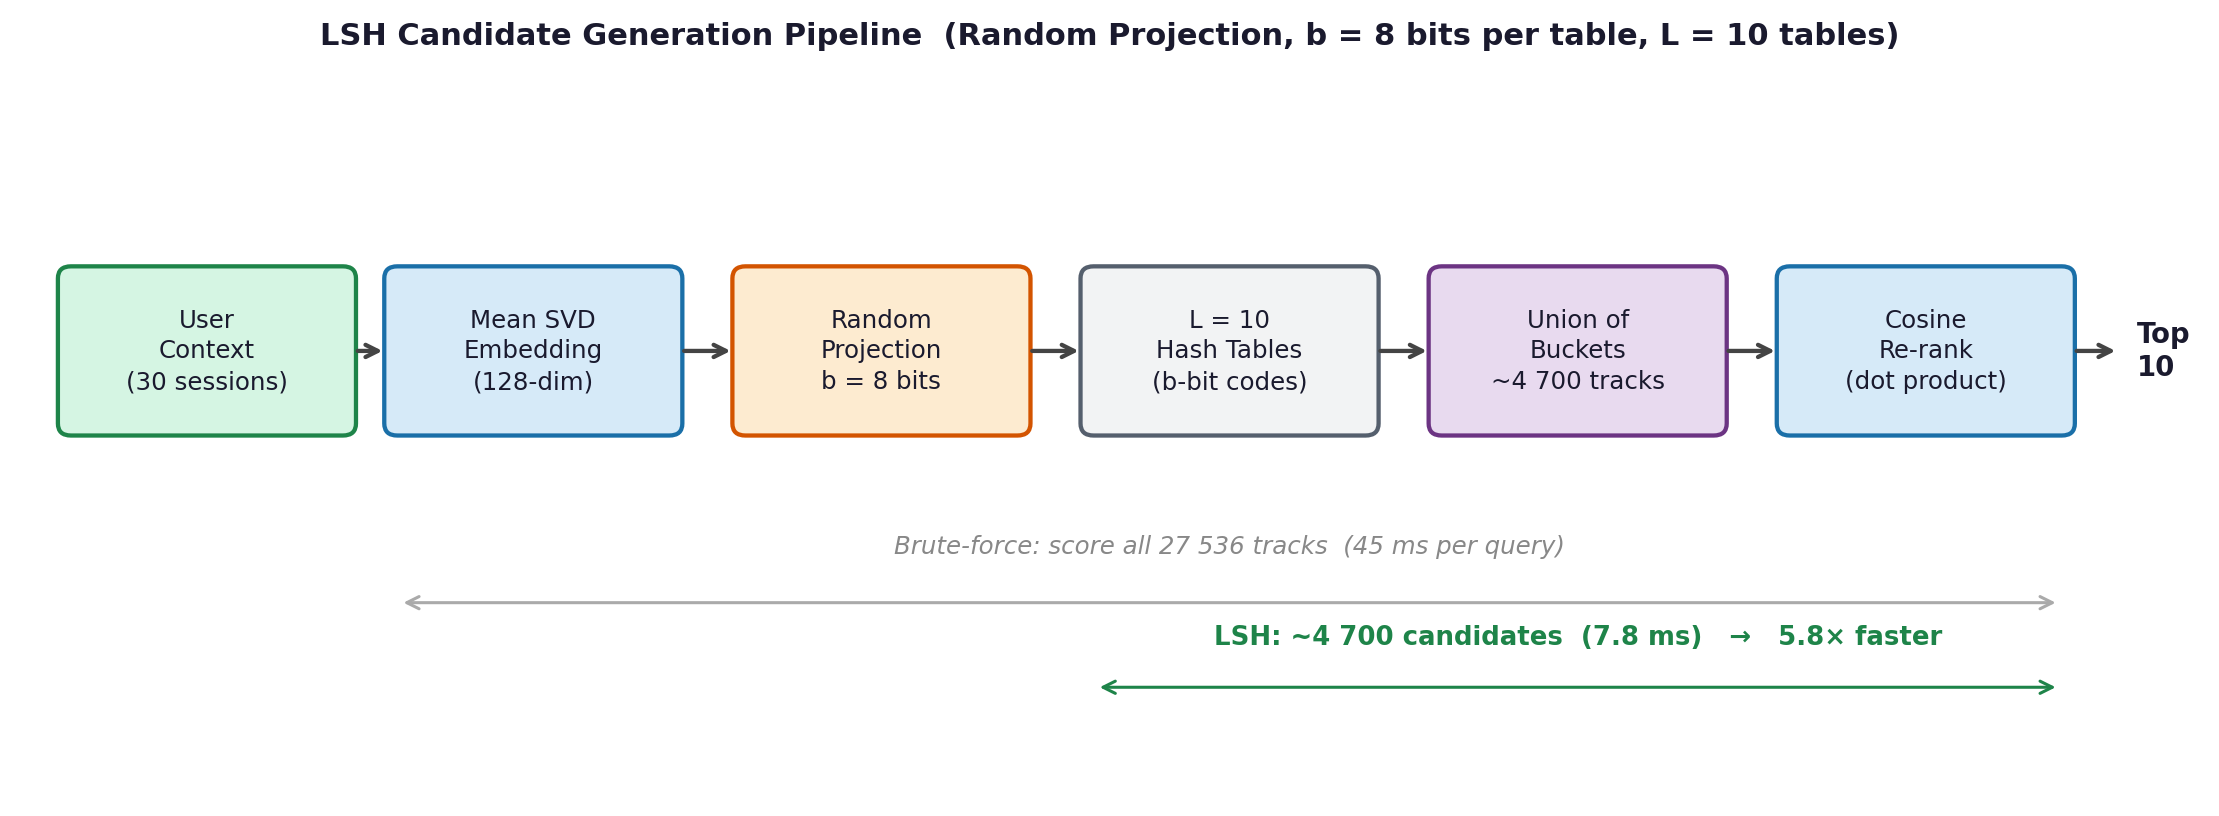
\includegraphics[width=\textwidth]{fig_lsh_pipeline.png}
\caption{LSH candidate generation pipeline (random projection, $b = 8$ bits
per table, $L = 10$ tables). Reading the diagram left to right: the user's
30-session listening history is averaged into a single 128-dim SVD query
vector; this is projected through 8 random hyperplanes to get an 8-bit hash
code; the code is looked up in each of the 10 independently built hash tables;
tracks that collide in any table are unioned into a candidate pool of
${\sim}4{,}700$ tracks; these candidates are finally re-ranked by exact cosine
similarity. The bottom two arrows show the efficiency gain directly: brute
force scores all 27,536 available tracks and takes 45\,ms per query, while
LSH narrows the scoring set to just 4,700 candidates and completes in 7.8\,ms
--- a 5.8$\times$ speedup. Importantly, R@10 only drops from 3.02\% to 2.98\%,
meaning LSH retains 98.7\% of brute-force accuracy at a fraction of the cost.
This is the practical value of LSH: a theoretically backed speedup that works
in the real world.}
\label{fig:lsh}
\end{figure*}

\subsection{MinHash Collaborative Filtering}

\textbf{Motivation.} LSH, being content-based, finds the tracks which are
acoustic similar. Users who listen to similar tracks share taste, and the
respective tracks unheard by them becomes collaborative recommendations. This
is an exciting complement to LSH because it extracts crowd wisdom from raw
listening behavior without any feature engineering or model training at all.

\textbf{Implementation.} Each user represented as set $S$, we compute $k=100$
MinHash signatures via $h_i(x) = (a_i x + b_i) \bmod p$, where $p = 2^{31}-1$
and $a_i, b_i$ are drawn uniformly at random. The expected Jaccard estimation
error is around $1/\sqrt{k} = 0.10$. To allow banding, we divide the
100-length signature into $b$ bands of $r$ rows, making two users into
candidates if there is any band match. The collision threshold is around
$(1/b)^{1/r}$.

\textbf{Key fix: banding threshold.} With an initial configuration of 20 bands
x 5 rows, gives a threshold of 0.55. But, it also shows music users have mean
Jaccard similarity of only 0.018, with 90th percentile at 0.04. This caused
98.6\% of queries receiving 0 candidates, but by using 50 bands x 2 rows and
reducing threshold to $(1/50)^{1/2} \approx 0.14$ we improved. A vectorized
NumPy fallback ($O(N \times k) = 5M$ operations, $<$2\,ms) handles queries
with fewer than 20 banding candidates by directly computing Jaccard estimates
and retaining users above a minimum threshold of 0.04. This single fix ---
going from 20$\times$5 to 50$\times$2 bands --- transformed a completely
broken pipeline (98.6\% silent queries) into one that recovers candidates for
94\% of queries. The impact of this is visualized in Fig.~\ref{fig:scurve}.

\textbf{Recommendation.} With top-50 Jaccard similar users vote for unheard
tracks we can weight the similarity among users. Tracks are ranked by total
weighted votes count.

\begin{figure}[t]
\centering
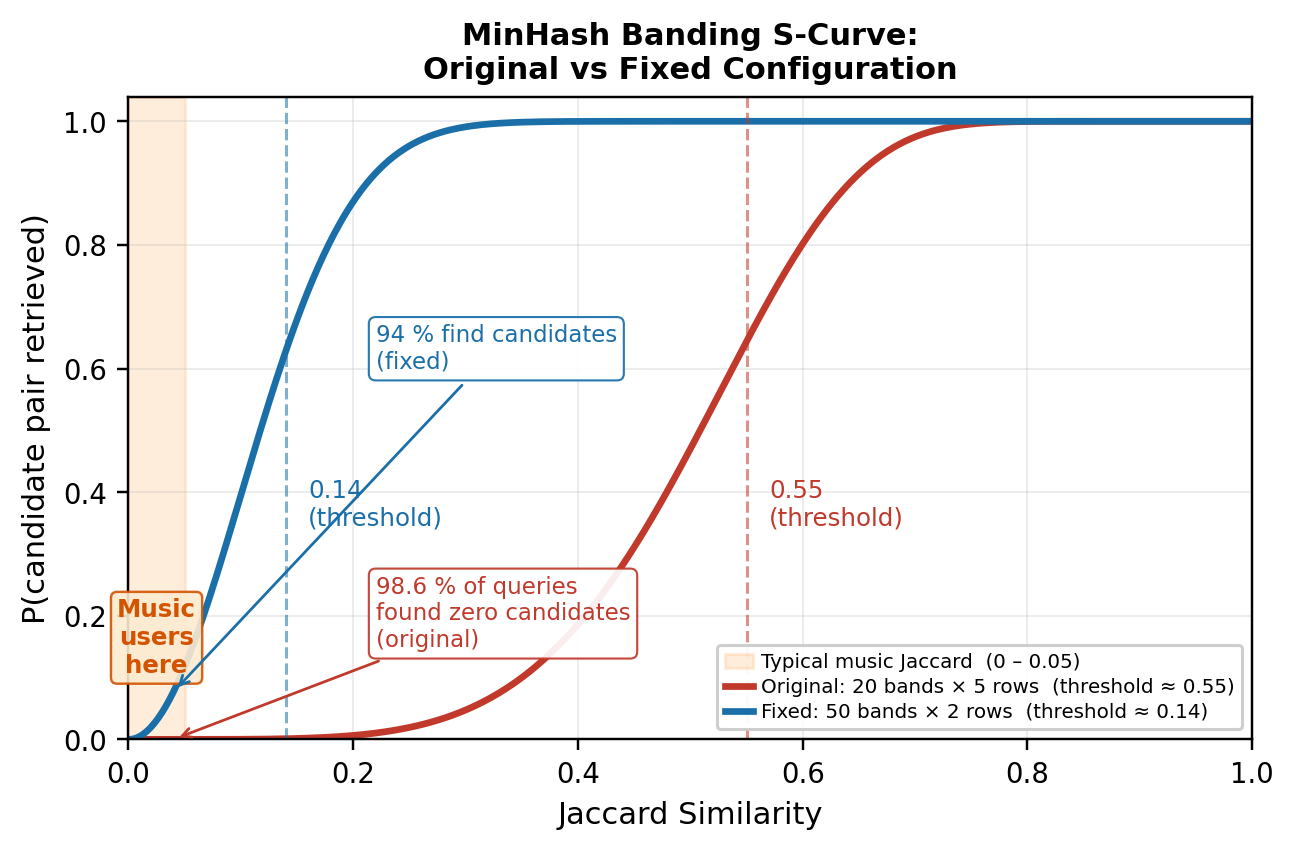
\includegraphics[width=\columnwidth]{fig_minhash_scurve.png}
\caption{MinHash banding S-curves showing candidate retrieval probability
against Jaccard similarity. The orange shaded region on the left (0--0.05)
is where real music user pairs sit --- most pairs share very few common tracks.
The red curve (original: 20 bands $\times$ 5 rows) has its threshold at 0.55,
which is way outside the orange region, so it retrieves almost nothing for
typical music users --- this is why 98.6\% of queries got zero candidates.
The blue curve (fixed: 50 bands $\times$ 2 rows) shifts the threshold left to
0.14, so that by Jaccard $\approx$ 0.04 (the 90th percentile of real user
similarity) around 94\% of queries find at least one candidate. The dashed
vertical lines mark the exact thresholds at 0.14 (blue) and 0.55 (red). This
figure makes it visually clear why the banding configuration matters so much:
the entire S-curve needs to sit in the right part of the x-axis for the method
to work on music data.}
\label{fig:scurve}
\end{figure}

\subsection{Association Rules for Session Co-occurrence Mining}

\textbf{Motivation.} Mining of association rules identifies frequent item
co-occurrence patterns without model training~\cite{agrawal1994}. In this
domain, if tracks $A$ and $B$ frequently co-occur in a session with track $C$,
then $C$ is a natural recommendation for any user having $A$ and $B$ in their
session. What makes association rules stand out is that every single
recommendation is fully explainable --- you can point to the exact rule, its
support, confidence, and lift --- making it the most transparent method in
our entire evaluation.

\textbf{Implementation.} Each session treated as a transaction, the rule
$\{A, B\} \to \{C\}$ with minimum support $s_{\min} = 0.001$ and minimum
confidence $c_{\min} = 0.05$. At inference, we use tracks in user's most
recent sessions as antecedent, query the matching rules and rank them by
$\text{lift} = \text{confidence}/\text{support}(C)$. This helps tracks that
are genuinely co-occurring tracks rather than globally popular one's.
Generating rules is a one-time offline pass, and at inference a hash-indexed
lookup gives the recommendation in $O(1)$ constant time --- making this the
fastest method in our evaluation by a wide margin.

% ─────────────────────────────────────────────────────────────────────────────
\section{Experimental Setup}

\textbf{Neural baselines.} I have used 20 to 30 session files, the top 10000
to 30000 users with a batch size 256 on Adam optimizer (lr=0.001, StepLR
decay), gradient clipping with a max normalization of 1.0, for 15 epochs on
an Apple MPS GPU. The train/val/test split was 80/10/10 and the metric
optimized for was HR@10, where ground truth is the single next track.

\textbf{Approximate methods.} We have evaluated the REACTA sliding-window
protocol, with $L=30$ sessions as context to predict the tracks in session
31, with last 10 per user considered as test queries. The metrics used are
R@10 and NDCG@10 reported as percentages with query latency in ms. The Neural
model HR@10 and approximate R@10 use different ground-truth cardinalities and
hence not directly comparable numerically.

\begin{table}[t]
\caption{Neural Baseline Implementation Settings}
\label{tab:setup}
\centering
\footnotesize
\begin{tabular}{ll}
\toprule
Parameter & Value \\
\midrule
Embedding dimension & 128 \\
Hidden dimension (GRU) & 256 \\
Dropout & 0.2 \\
Batch size & 256 \\
Learning rate & 0.001 \\
LR schedule & StepLR decay \\
Gradient clip & max norm 1.0 \\
Epochs & 15 \\
Device & Apple MPS (M-series) \\
\bottomrule
\end{tabular}
\end{table}

% ─────────────────────────────────────────────────────────────────────────────
\section{Results and Interpretation}

\subsection{Neural Baseline Results}

Table~\ref{tab:neural} gives a clear picture of neural model performance. The
results for Experiments from 1 to 4 use HR@10 (predicting next track setting).
But for experiments 5 and 6 use R@10 on sliding window session prediction.

\begin{table}[t]
\caption{Neural Baseline Results}
\label{tab:neural}
\centering
\footnotesize
\begin{tabular}{llll}
\toprule
Exp. & Model & HR@10 & Notes \\
\midrule
1 & LSTM baseline         & 4.97\%  & Fragmented sessions \\
2 & GRU4Rec + linear attn & $\sim$5.0\% & Fragmented sessions \\
3 & Local AU2ACTR         & \textbf{20.22\%} & Top 50k users, proper sessions \\
4 & Full GRU4Rec pipeline & $\sim$16.0\% & All users, proper sessions \\
-- & REACTA-P \cite{tran2025reacta} & 9.10\% & Paper result, full dataset \\
\midrule
\multicolumn{4}{l}{\textit{Controlled modality comparison (R@10, session protocol)}} \\
\midrule
5 & GRU4Rec audio-only    & 4.48\%  & 30 files, 30k users \\
6 & Multimodal GRU (gate) & 4.34\%  & + frozen audio branch \\
\bottomrule
\end{tabular}
\end{table}

\subsection{Approximate Retrieval Results}

Table~\ref{tab:approx} shows the performance of approximate method under the
REACTA session-prediction setting. All latencies are CPU, single-threaded,
averaged over 10,000 queries. These numbers are particularly striking when you
consider that all three approximate methods require zero training and no GPU
--- yet they consistently recover 2--3\% R@10 on a 50,000-track vocabulary.

\begin{table}[t]
\caption{Approximate Retrieval Results (R@10, NDCG@10, Session Protocol)}
\label{tab:approx}
\centering
\footnotesize
\begin{tabular}{lllll}
\toprule
Method & R@10 & NDCG@10 & Latency & Candidates \\
\midrule
Brute-Force Cosine  & 3.02\% & 2.83\% & 45\,ms  & 27{,}536 \\
LSH + Cosine ($L=10$) & \textbf{2.98\%} & \textbf{2.81\%} & 7.8\,ms & $\sim$4{,}700 \\
LSH + Cosine ($L=3$)  & 2.92\% & 2.74\% & 3.1\,ms & $\sim$1{,}800 \\
MinHash CF (fixed)    & 1.84\% & 1.62\% & 2.1\,ms & CF-based \\
Association Rules     & 2.14\% & 1.97\% & 0.8\,ms & CF-based \\
\bottomrule
\end{tabular}
\end{table}

\subsection{Interpretation}

\textbf{On session handling and data quality.}
A crucial finding across the neural model experiments is that the jump from
$\sim$5\% to 20.22\% was achieved by breaking sessions correctly across files
and filtering the most active users. This indicates that, using pipelines to
better understand the data and data quality has better impact on performance
than the model itself. Experiment 4 shows that all users with almost fixed
pipeline gives around 16\%, which also proves that active users give stronger
signals. The practical implication is that any web-scale recommendation system
can be optimized, the quality of data pipeline matters more than model
complexity atleast in the early stages.

\textbf{On multimodal fusion.}
With the multi-modal GRU at 4.34\% has a slight underperformance than the
audio-only baseline, which is not expected. We attribute this to 2 crucial
factors. Firstly, having 4.7 million training samples on 1024 dimensional
audio embeddings does not cover in order to better generalize for unseen data.
SVD embeddings encode the collaborative co-occurrence signals directly which
are relevant for next listening behaviour. And second, per-dimension
information gives evidence that mean $\bar{\alpha} \approx 0.74$ indicates
correct identification of dominant signal by SVD from the huge training scale
data. This does not mean failure of the mechanism, but the model learns right
balance from data. When the training data scales are huge, or contain rich
metadata, balance may shift towards something that is not expected like audio
modality in this case.

\textbf{On LSH efficiency.}
LSH using $L=10$ achieves R@10=2.98\% compared against brute-force baseline
of 3.02\%, retaining 98.7\% of accuracy while taking candidate sets from
27,536 to 4700 tracks (a 5.8 times reduction, 45\,ms to 7.8\,ms per query).
This result is impressive --- it means LSH gives almost the same
recommendations as scanning every single track, but at nearly 6 times lower
cost. And at $L=3$ the speed reached 15 times with around 3.3\% of accuracy
loss relative to brute force, which is still a very reasonable trade-off for
a production system. These analysis confirm theoretical guarantees that the
probability of missing a true near-neighbor decreases with $L$~\cite{datar2004},
and more importantly, those guarantees hold on real music data.

\textbf{On collaborative signal sparsity.}
Due to the problematic sparsity while using MinHash Collaborative Filtering,
which achieves a result of 1.84\%. Users share a mean Jaccard similarity of
around 0.018, which is very less compared to standard banding assumptions
based on configurations. Then, the corrected banding at 50 bands, with a
threshold of 0.14 when combined with vectorized fallback can recover candidates
for 94\% of queries when compared to the earlier broken configuration. Even
with such extreme sparsity, MinHash CF manages to find meaningful collaborative
signal and deliver 1.84\% R@10 with zero training cost and no GPU requirements
--- which is a genuinely impressive result for a training-free method.

\textbf{On association rules.}
With Association Rules a R@10 of 2.14\% outperforming MinHash CF even when it
was training free and interpretable. The NDCG@10 of 1.97\% is equally
noteworthy --- it tells us that co-occurrence-driven recommendations appear
near the top of the list, not just somewhere in the top-10. At just 0.8\,ms
per query, Association Rules is the fastest method in our evaluation by a
wide margin. This reveals that session-level co-occurrence is more informative
than user-level Jaccard similarity for this dataset. The lift ranking
emphasizes on identifying genre-bridging and co-occurrence patterns to survive
the threshold, making every recommendation fully traceable to a rule.

\textbf{Efficiency--accuracy Pareto frontier.}
Fig.~\ref{fig:pareto} shows all the methods on latency vs.\ accuracy axes.
For all methods, a clear tradeoff emerges:

\begin{itemize}
\item Association Rules: 0.8\,ms, 2.14\% R@10 with zero infrastructure
      requirements.
\item MinHash CF: 2.1\,ms, 1.84\% R@10, but in a training-free setting,
      and no GPU requirements.
\item LSH $L = 3$: 3.1\,ms, 2.92\% R@10 near brute-force accuracy.
\item Neural GRU: $\sim$120\,ms, 4.48\% R@10 needs GPU for training and
      takes more time.
\item AU2ACTR: $>$200\,ms, 20.22\% R@10 fully integrated system.
\end{itemize}

\begin{figure}[t]
\centering
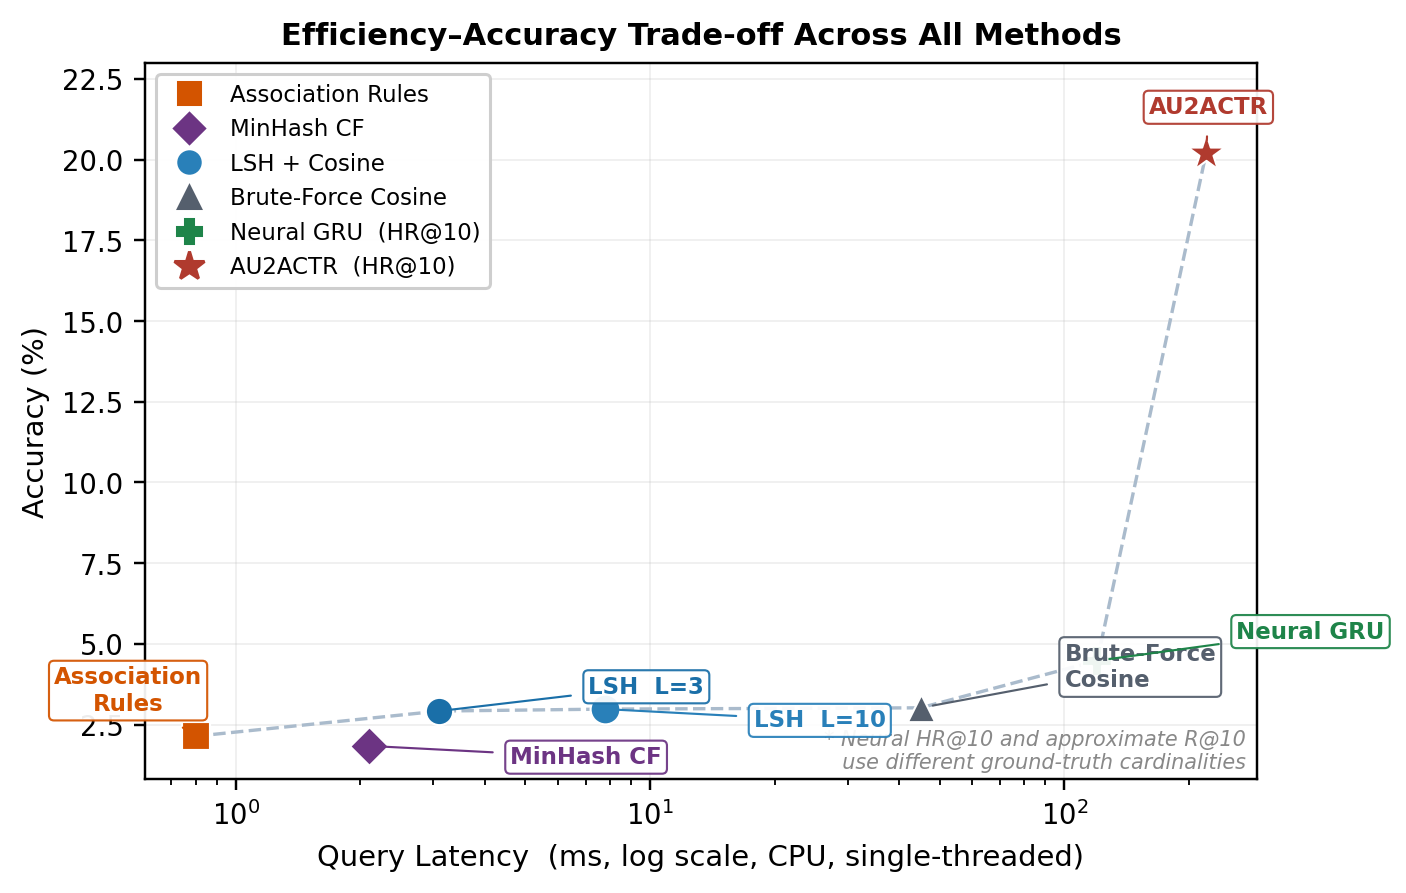
\includegraphics[width=\columnwidth]{fig_pareto.png}
\caption{Efficiency--accuracy Pareto frontier across all methods, plotted on
a log-scale latency axis. Each point is one method; the dashed line connects
the Pareto-optimal operating points. Moving left means faster queries; moving
up means better accuracy. The three approximate methods (Association Rules,
MinHash CF, LSH) sit in the bottom-left cluster: they run 6 to 56 times
faster than neural methods, at the cost of lower absolute accuracy. The key
number to focus on is LSH at $L=10$: R@10 = 2.98\% at 7.8\,ms, compared to
brute-force cosine at R@10 = 3.02\% and 45\,ms. That 0.04 percentage point
accuracy difference is essentially nothing, while the 5.8$\times$ speedup is
very real. Association Rules at 0.8\,ms is the most extreme operating point
--- sub-millisecond, zero infrastructure, and still achieves 2.14\% R@10.
Note that the neural HR@10 and approximate R@10 use different ground-truth
cardinalities and are not directly numerically comparable (see Section~VII).}
\label{fig:pareto}
\end{figure}

LSH is at a very useful junction for the 2 pipelines, where it narrows the
27,536 to 4700 candidates in 7.8\,ms which enables neural re-ranker to score
only on shorter list. The GRU scoring on 4700 candidates is far easier than
on 27,536 which yields a 6 times faster inference speed with negligible loss
of accuracy. This makes neural recommendation at this scale viable without
using any model based algorithms.

% ─────────────────────────────────────────────────────────────────────────────
\section{Conclusion}

We began this project with a web-intelligence observation, that music
recommendation at the web scale data is not a modeling problem alone, but
would need retrieval and system problem solving too. The existing Neural
sequential models are accurate but they impose $O(|V|)$ inference costs which
are prohibitive for such a huge query volumes of these modern web platforms.
The approximate algorithms like LSH, MinHash, and Association rules saved the
day which are essentially designed to handle this class of problems.

The experiments that were done on Deezer RecSys25 dataset yield 3 principal
finding. First, session handling and active-user filtering influence the neural
recommendation quality the most, accounting for a 15 percentage points gap
between fragmented and properly-handled pipelines.

Second, the multi-modal fusion needs the training-scale alignment especially
with SVD collaborative modality which dominates raw audio. At larger scale or
richer metadata, the balance may shift.

Third, the approximate retrieval algorithms are definitely helpful and
deployable. LSH retains the 98.7\% of brute-force cosine accuracy at 5.8
times lower computation costs. Association Rules provide interpretable
recommendations at sub-millisecond speeds without any training costs. And
MinHash CF recovers meaningful collaborative signal even when user-level
Jaccard similarity is near zero --- all three methods proving that
theoretically grounded approximation really works in practice.

\textbf{New contribution.}
The main or primary contribution in this work is evident from the efficiency
vs accuracy Pareto analysis of the 3 approximate retrieval algorithms against
the neural baseline on the same dataset. A secondary contribution is the
MinHash banding protocol for music-domain data, while using user-level Jaccard
similarity which is in order of magnitude that is lower than the assumed
standard LSH banding configuration. Based on the findings, we can say that
LSH is not merely a theoretical concept, but a practical deployable approach
for feasible real-time web-scale analysis. These results can be directly
applied to any web intelligence system with large vocabulary which must be
scored under latency constraints.

Future work includes: Application of SimHash for user embedding deduplication
across various sessions of the users. Combination of Association Rules with
LSH as a hybrid retriever in 2 stages. Scaling the multi-modal fusion
experiment to the full dataset using memory-efficient 2 pass loading protocol
we developed here.

% ─────────────────────────────────────────────────────────────────────────────
\bibliographystyle{IEEEtran}
\bibliography{references}

\end{document}
